\documentclass[11pt,a4paper]{report}

% Aberstwyth dissertation LaTeX Template
% Authors: Dr. Hannah Dee (hmd1@aber.ac.uk), Neil Taylor (nst@aber.ac.uk)
% This has been adapted from the Leeds Thesis template and the 
% Group Project template for Computer Science in Aberystywth University.
% 
% All comments and suggestions welcome.
%
% Template designed to be used with pdflatex: it may need alteration to
% run with a different LaTeX engine

% To build document on the unix command line, run four commands:
 
% pdflatex dissertation
% bibtex dissertation
% pdflatex dissertation
% pdflatex dissertation

% you will end up with dissertation.pdf 
\usepackage{mmp}

% the following packages are used for citations - You only need to include one. 
%
% Use the cite package if you are using the numeric style (e.g. IEEEannot). 
% Use the natbib package if you are using the author-date style (e.g. authordate2annot). 
% Only use one of these and comment out the other one. 
\usepackage{cite}
%\usepackage{natbib}

% Use the following to selectively exclude chapters
%\includeonly{cover,abstract,acknowledge,declare,chapter1,chapter2}
\usepackage{pdfpages}

\begin{document}

% all of the include directives below refer to tex files
% so 
\title{Mobile Vision Based Risk Detection:
Using computer vision to detect potential risks in a
Parrot AR.Drone 2.0}

% Your name
\author{Joseph James}

% Your email 
\authoremail{jgj2@aber.ac.uk}

\degreeschemecode{G400} %e.g. G400 
\degreeschemetitle{Computer Science} % e.g. Computer Science
\degreetype{BSc}

\modulecode{CS39440} % i.e. CS39440, CC39440, CS39620
\moduletitle{Major Project} % i.e. Major Project or Minor Project

\date{} % i.e. the date of this version of the report

\status{Release} % Use draft until you create the release version. Then, change this to Release.
\version{1.0}
%The title and name of your supervisor.
\supervisor{Dr. Myra Wilson} 

%The email for your supervisor. 
\supervisoremail{mxw@aber.ac.uk}

\maketitle



 includes cover.tex - to change the content,
% edit the tex file

\pagenumbering{roman}

% This is the front page

\title{Mobile Vision Based Risk Detection:
Using computer vision to detect potential risks in a
Parrot AR.Drone 2.0}

% Your name
\author{Joseph James}

% Your email 
\authoremail{jgj2@aber.ac.uk}

\degreeschemecode{G400} %e.g. G400 
\degreeschemetitle{Computer Science} % e.g. Computer Science
\degreetype{BSc}

\modulecode{CS39440} % i.e. CS39440, CC39440, CS39620
\moduletitle{Major Project} % i.e. Major Project or Minor Project

\date{} % i.e. the date of this version of the report

\status{Release} % Use draft until you create the release version. Then, change this to Release.
\version{1.0}
%The title and name of your supervisor.
\supervisor{Dr. Myra Wilson} 

%The email for your supervisor. 
\supervisoremail{mxw@aber.ac.uk}

\maketitle



                        

% Set up page numbering
\pagestyle{empty}

% declarations of originality 
\thispagestyle{empty}

%%%
%%% You must sign the declaration of originality. 
%%%
\begin{center}
    {\LARGE\bf Declaration of originality}
\end{center}

In signing below, I confirm that:

\begin{itemize}
\item{This submission is my own work, except where 
clearly indicated.}

\item{I understand that there are severe penalties for 
Unacceptable Academic Practice, which can lead to loss 
of marks or even the withholding of a degree.}
 
\item{I have read the regulations on Unacceptable Academic 
Practice from the University's Academic Quality and 
Records Office (AQRO) and the relevant sections of the 
current Student Handbook of the Department of 
Computer Science.}
 
\item{In submitting this work I understand and agree to 
abide by the University's regulations governing these issues.}
\end{itemize}

\vspace{2em}
Name ........ Joseph James ........ \\

\vspace{1em}
Date  ........ 04/05/2016 ........\\

%%% 
%%% We would like to make a selection of final reports available to students that take 
%%% this module in future years. To enable us to do this, we require your consent. You 
%%% are not required that you do this, but if you do give your consent, then we will have 
%%% the option to select yours as one of a number of reports as examples for other 
%%% students. If you would like to give your consent, then please include the following 
%%% text and sign below. If you do not wish to give your consent, please remove this 
%%% from your report. 
%%%
\vspace{1em}
\begin{center}
    {\LARGE\bf Consent to share this work}
\end{center}

In signing below, I hereby agree to this dissertation being made available to other
students and academic staff of the Aberystwyth Computer Science Department.  

\vspace{2em}
Name ............................................................  \\

\vspace{1em}
Date ............................................................ \\


               

\thispagestyle{empty}

\begin{center}
    {\LARGE\bf Acknowledgements}
\end{center}

I'd like to thank Dr. Myra Wilson for her help in supervising me throughout this project.

I'm also grateful to Phil Charleswoth from Airbus for providing access to the Parrot AR Drone 2.0.
 % Acknowledgements
0\thispagestyle{empty}

\begin{center}
    {\LARGE\bf Abstract}
\end{center}
This project aims to implement vision based autonomous object avoidance within a monocular quad-copter in order to provide autonomous assistance to those hard of sight. Using Harris Corners  I detect features, then track these features using Lucas-Kanade optical flow. These interest points are then used to predict background motion/camera motion via a RANSAC generated homography. After this, the outlying interest points are clustered together based on their motion vectors/motion vector angles using an agglomerative hierarchical clustering technique. These clusters are then refined using k-Nearest Neighbours, after which the clusters are ensured to be consistent throughout the video feed. Each cluster is then used as an object and it is determined whether or not it is a risk to be avoided, if it is it's position is used to allow the drone to avoid the object.                 % Abstract

\pagenumbering{roman}
\pagestyle{fancy}
\fancyhead{}
\fancyfoot[C]{\thepage}
\renewcommand{\headrulewidth}{0 pt}
\renewcommand{\chaptermark}[1]{\markboth{#1}{}}

\tableofcontents   
\newpage

% Set up page numbering
\pagenumbering{arabic}

\setchapterheaderfooter

% include the chapters
\chapter{Background \& Objectives}
\vspace{-20pt}
%This section should discuss your preparation for the project, including background reading, your analysis of the problem and the process or method you have followed to help structure your work.  It is likely that you will reuse part of your outline project specification, but at this point in the project you should have more to talk about. 

%\textbf{Note}: 

%\begin{itemize}
%   \item All of the sections and text in this example are for illustration purposes. The main Chapters are a good starting point, but the content and actual sections that you include are likely to be different.
   
%   \item Look at the document on the Structure of the Final Report for additional guidance. 
   
%\end {itemize}
\section{Background \& Analysis}
%What was your background preparation for the project? What similar systems did you assess? What was your motivation and interest in this project? 

%  BACKGROUND
%    - Checked out drones, how they fly in general and what kind of things is possible.
%    - Checked out specifically the AR Drone 2.0 +  it's capabilities
%      - How to control it?
%        -ROS, the C library it was provided with, .js nodes, CVDrone.
%    -Vision stuff
%      - Monocular vision for object detection
%      - Using a single camera for determining depth of objects (Not totally necessary for me, unknown at the time)
%    - Other projects with the AR Drone.
%

\subsection{Drone capabilities}
The platform for this project was the Parrot AR.Drone 2.0, which is a quad-copter with limited sensor capabilities. Before this project could be pursued these capabilities had to be fully assessed to understand the limits of the quad-copter, ensure the project was possible and to limit the scope of the project.


\subsubsection{Cameras}
The first camera is a high quality front-facing camera, traditionally used to take pictures or help a user guide the quad-copter when it isn't in line of sight. The front facing camera has a maximum 720p resolution with a 30fps frame rate and a 92$^{\circ}$ viewing angle. In a vision based navigation system this would be the camera in use, as it has the best view of potential collisions and objects in the path of the drone. It also has a higher resolution, which will improve our features but also increase computation time although the effects of the increased computation is likely to be negligible.

The second camera is a downward facing camera which is mainly used to calculate ground speed within the drone but it can be used to take pictures by the user. This second camera is a Quarter Video Graphics Array with a resolution of 320 x 240.  While this camera would not be able to be used in a navigation system due to it's orientation, it could be used in other vision projects such as mapping from above or navigating using pre-planned flight instructions from signs on the floor.


\subsubsection{Processor + RAM}
The on-board processor of the AR Drone 2.0 is a 1GHz 32 bit ARM Cortex A8 processor. This processor is not available to the user without altering the firmware that is directly on the drone. If this route were to be followed, a lot of safety features would have to be re-written, along with software to directly control the motors in the drone and software to accept commands from elsewhere. This would be out of scope for a project of this size, so the best alternate solution is to perform processing elsewhere. Due to the higher processing power available elsewhere, this is likely more beneficial for a vision based system.


\subsubsection{Connectivity}
In order to connect to the quad-copter from a separate device, the drone has a wireless access point. This wireless access card allows for connection to B/G and N connections, meaning it can go up to 100Mb/s \cite{Nstandard} Connection speed however could be an issue, slowing down transmission of images from the drone and commands to the drone.

 To properly assess this potential bottleneck, the time taken to transfer 100 packets of information to the drone and back was taken and averaged via the "ping" command in a terminal when connected to the drone. This connection speed average is shown in figure 1, the outliers are likely to produce freezes within the program and vision calculations, so some robustness in our implementation will be needed to deal with this.

\begin{figure}
\centering
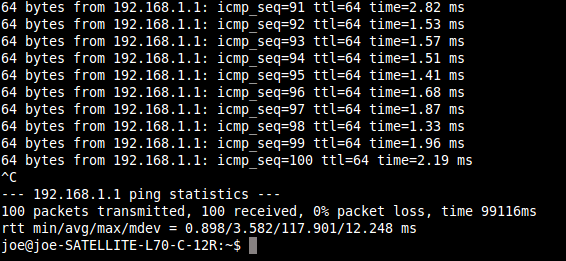
\includegraphics[scale=0.5]{PingScreen.png}
\caption{The results of the ping command when connected to the AR Drone 2.0}
\end{figure}
\subsubsection{Other sensors}
\begin{itemize}
  \item 3 axis gyroscope 2000°/second precision
  \item 3 axis accelerometer +-50mg precision
  \item 3 axis magnetometer 6° precision
  \item Pressure sensor +/- 10 Pa precision
  \item Ultrasound sensors for ground altitude measurement
\end{itemize}


\subsection{Drone control}
Being able to control the drone is another important aspect of this project, as the project is not possible without at least access to the camera feeds. There are a couple of important factors that needed to be considered for this part of the background research such as language, ease of use, ease of implementation, feature availability and licenses.


\subsubsection{AR Drone SDK}
This is the Source Development Kit provided by the developers of the AR Drone 2.0\cite{DroneAPI}, provided in C with extensive documentation\cite{DroneDevGuide}. This, however, is very confusing to read and made it quite difficult to follow and implement. Coupled with inexperience with C, drones and computer vision, the project would have been made much harder using this software to control the drone. The SDK is provided under Parrot's own license, included in Appendix A.


\subsubsection{Node Copter}
This is a JavaScript based control software, provided here\cite{nodecop}. Having used Java before, JavaScript would be easier to learn quickly. There are also libraries available to perform computer vision however they seemed to be inconsistent with their features, as I was unable to find a full implementation of OpenCV. Not knowing the exact algorithms that were going to be used for the vision meant this wasn't an option at the time.


\subsubsection{Robot Operating System Driver}
ROS is a collection of frameworks provided for use with Robotics, in this case a driver provided for the AR Drone 2.0\cite{ROSDrone}. The full extent of the capabilities of the driver are unknown to me, as learning ROS would have been very time consuming in this time constrained project and I decided not to continue this line of investigation.


\subsubsection{CVDrone}

CVDrone is software that combines control of the AR Drone 2.0 with OpenCV, an open source computer vision library\cite{CVDrone}. This software provides an API for C++, with easy to read documentation and example code. It's distributed under the GNU Lesser General Public License\cite{GNULGPL} and was the final choice for controlling the drone.  This was an easy choice, as it already contained the full OpenCV vision library as well as providing an easy to understand and learn method of implementation.

CVDrone acts as middleware between the project I am creating and the drone, giving me access to an API that allows for simple commands to be sent such as "takeOff()", "landing()" and "move3d(x, y, z, r)". This makes moving the drone a much easier task, simplifying what could have been an entire project itself into a few API calls. This software also provides access to OpenCV libraries by default, this isn't necessary and includes parts of OpenCV we won't need but does save time in implementing them as separate libraries.

Another small benefit of CVDrone is that it fixes an orientation issue within the original SDK for the AR Drone, flipping the Z axis so that as the value increases the drone flies up rather than down. This is a minor issue but it does avoid some confusing Z values.

\subsection{Vision}
While familiar with theory, implementation and more complicated theory had to be researched to gain a fuller understanding of what is possible within a moving, monocular system.


\subsubsection{Monocular vision}
One of the main issues facing a vision based obstacle avoidance system is a lack of depth inherent in a single camera system. Depth perception from a single camera is a difficult problem, as depth is usually determined through the calculation of disparity between two images of the same area from a slightly different perspective \cite{StereoDepth}. However this becomes less of an issue within a moving system and a monocular system can even be used for 3D mapping of objects using optical flow\cite{3DMapOpFlowMono} in this case.

This indicates to me that it's possible to implement a system that will provide sufficient obstacle avoidance ability within the drone.

\subsubsection{Monocular obstacle avoidance}
Further research into monocular obstacle avoidance found papers referencing how optical flow is used biologically in flying insects\cite{citeulike:9515178} and birds\cite{opticalFlowBirds}. This gave me the idea of using the phenomenon of relative motion to avoid obstacles that are closer to the camera and led to research further in the direction of using optical flow rather than depth mapping.

 In the search for optical flow based obstacle avoidance, the papers \cite{souhila2007optical} and \cite{PhoneObstacleAvoidance} seemed relevant in achieving the projects goals. \cite{PhoneObstacleAvoidance} was closer to the original intent in using optical flow and final goal of the project and as such became the basis for this project.
 
 The paper describes a method of finding, classifying and then warning about objects within a moving monocular system using computer vision. For this project however, we only needed to be able to identify and avoid objects within the drones view. \S3.1 of the paper details 7 steps to identify obstacles in the path of the camera and whether or not they should be avoided. A summary of these 7 steps is shown below:
\begin{description}
	\item [Step 1 - Interest Point Extraction] In this step, features are detected and turned into interest points. In the paper, the interest points are detected using a grid sampling method in order to allow for equal spread of features throughout the image. This means that less textured regions of the image still factor in to steps further down the line.
	
	\item[Step 2 - Interest Point Tracking] Here, the interest points from step 1 are taken and the Lucas-Kanade \cite{Lucas_KanadeOF} optical flow algorithm is applied to track them through multiple frames. Motion vectors, magnitude and angle of motion are all calculated within this step as well, which will be used later.
	
	\item[Step 3 - Camera/Background motion estimation] Now that interest points are being tracked, background motion/camera motion is estimated.
	
	This is done by generating a 3 x 3 homography using a robust RANSAC method and then multiplying this homography by the original points in order to produce an estimate position of the point in the next frame. The estimated point position is then compared to the actual point position, if the estimation error is larger than a particular threshold then the point is considered foreground.
	
	\item[Step 4 - Motion Classes estimation] These foreground points are then clustered together based using a hierarchical agglomerative technique on their motion magnitude and angular deviation from each cluster centroid. This is done in 2 phases. 
	
	The first phase sorts the interest points in descending order based on the number of occurrences of their motion vector angle. Then a new cluster is formed using the first interest point's motion vector angle as it's centroid.
	
	The second phase then calculates the remaining interest points motion magnitude and angular deviation from the cluster centroid. If the motion magnitude is equal to the centroid point and the angular deviation is beyond a certain threshold, the next interest point is added to that cluster. Otherwise, that interest point becomes the centroid for a new cluster. This is applied recursively until all points are part of a cluster.
	
	\item[Step 5 - Refinement of clusters/Interest Point refinement] Once the points are clustered, they're refined by applying a k-Nearest Neighbours algorithm. Each point is clustered again using k-NN with the Euclidean distance, if at least half of it's nearest neighbours do not belong to the same motion class, the point is removed from the cluster.
	
	\item[Step 6 - Motion Classes' temporal consistency] Now the clusters are refined, we memorise their trajectory over the past few frames and predict the position of the cluster. This is in order to protect clusters against partial occlusion, noise and image distortion.
	
	\item[Step 7 - Obstacle relevance establishing] Finally, the objects nature relevant to the camera is established. If the object is moving towards the cameras focus point, it is classed as {\em approaching}, otherwise it is classed as {\em departing}. Then a polar grid is projected onto the image and if the object is within a certain range, it is classed as {\em urgent}. Otherwise, the object will be classified as {\em normal}.
\end{description}

%i.e  dense interest points, fuzzyRansac, Multiple view geometry, agglomerative heirarchichal clustering, polar grids + focal points of cameras.
\subsubsection{Further reading}
This paper also introduced multiple concepts that needed further research to gain a proper understanding of the methods employed by the paper. These new concepts were Grid sampling of dense interest points, homography generation using RANSAC, polar grids and calculating the focal point of a camera.

\begin{description}
	\item [Grid sampling of dense interest points] For research on this topic, the paper "Dense Interest Points"\cite{DenseInterest} was a great help, providing an insight to the idea of sampling many interest points from an image. OpenCV does allow for multiple methods of extracting features and some of these techniques are classified as "Dense" techniques.]
	
	\item [Homography generation] The paper required the use of homographies to predict future locations of points and it did so through the use of a method called fuzzy RANSAC. A homography is generally kept in the form of a matrix and is used to relate 2 images from the same camera that have been taken from a different angle. This can be done using a regular RANSAC method, however in our paper it's done with a more robust version.
	
	\item[Fuzzy RANSAC] This is a method of implementing RANSAC that uses fuzzy logic to help classify the sample set into 3 sets: Good, vague and bad. RANSAC is then only applied only to the good sample set, which improves the robustness of the algorithm.

\end{description}

\subsubsection{OpenCV}
Having never used OpenCV one of the main background research points was learning how to use and implement OpenCV into my own applications. As part of this research I looked at example code provided with OpenCV and developed some simple implementations of basic vision on camera feeds to be certain I understood how to use the libraries correctly.

This also allowed for further understanding of OpenCV's data types that are used such as cv::Mat and cv::Point2f, Matrixes and float 2D Points respectively, as well as a little practice with C++ before the main project.

The choice to use OpenCV is a clear one, as it's one of the largest, fully featured computer vision libraries available and is provided fully for the C++ language. The open source nature of OpenCV also helps improve understanding of what's happening behind the scenes, which will potentially help improve the time frame of understanding OpenCV for the project. OpenCV is also extensively documented and has a large number of users, meaning that problems will be quicker to solve than if a more obscure library were being used.

\subsection{Tasks to be undertaken and where they came from}

The paper \cite{PhoneObstacleAvoidance} breaks down the overall structure of this problem quite well, making most of the visions steps into specific tasks. It doesn't cover the entire project however, as adaptations needed to be made to get the vision to interact with the drone as well as a drone controller. 

This essentially means that there are 2 major parts to this project, Vision and Drone control.

\subsubsection{Vision}
The paper splits the vision into 7 steps, so initially these 7 steps were used as tasks to be completed, however they were too large to be considered stories in my methodology. In order to help fit them into my methodology, I considered most steps an "Epic", consisting of multiple stories. The only exception to this was the feature detection, feature tracking through frames and interest point refinement, as these steps were small enough to be considered stories of their own right. A break down of each epic follows:

\begin{description}
	\item[Epic 1 : Camera/background motion estimation] Step 3 of 7.\\
	\vspace{-15pt}
	\begin{itemize}
		\item Homography generation
		\item Prediction of point placement in future frames
		\item Classify points based on estimation error
	\end{itemize}
	\item[Epic 2 : Motion Classes estimation] Step 4 of 7.\\
	\vspace{-15pt}
	\begin{itemize}
		\item Sort motion vectors in descending order based on number of occurences
		\item Classify each point using agglomerative hierarchical clustering
	\end{itemize}
	\item[Epic 3 : Motion classes' temporal consistency] Step 6 of 7.\\
	\vspace{-15pt}
	\begin{itemize}
		\item Store motion class centroids trajectory over N past frames.
		\item Predict position of the object compensated with camera/background motion.
	\end{itemize}
	\clearpage
	\item[Epic 4 : Relevance establishing] Step 7 of 7.\\
	\vspace{-15pt}
	\begin{itemize}
		\item Find cameras focal point
		\item Classify objects as approaching or departing based on the trajectory of the motion class
		\item Implement a polar grid projection
		\item Classify objects as Urgent or Normal, based on distance from drone.
	\end{itemize}
\end{description}

\subsubsection{Drone control}
This section is the part of the project that relates to controlling the drone and tying it in to the vision system above. While the vision system is considered a collection of Epics, the drone controller can be considered an Epic in itself, as it's not the main component of this project. The drone controller acts as a method of implementing the vision into a robotics system, rather than being a main focus of work.

\begin{description}
	\item[PID controller] Here we implement a PID controller, which will be the main part of the controller, allowing for 
	\item[API for drone control] This story is all about implementing a method of communicating direction to the drone, as CVDrone only provides move3d(x, y, z, r) where x, y, z and r are velocities. 
\end{description}
%\section{Analysis}
%Taking into account the problem and what you learned from the background work, what was your analysis of the problem? How did your analysis help to decompose the problem into the main tasks that you would undertake? Were there alternative approaches? Why did you choose one approach compared to the alternatives? 

%There should be a clear statement of the objectives of the work, which you will evaluate at the end of the work. 

%In most cases, the agreed objectives or requirements will be the result of a compromise between what would ideally have been produced and what was felt to be possible in the time available. A discussion of the process of arriving at the final list is usually appropriate.

%i.e explain our process (personal kanban/scrum)
\clearpage
\section{Process}
%You need to describe briefly the life cycle model or research method that you used. You do not need to write about all of the different process models that you are aware of. Focus on the process model that you have used. It is possible that you needed to adapt an existing process model to suit your project; clearly identify what you used and how you adapted it for your needs.
%==============================================================================

%==============================================================================
For this project, a methodology was followed in order to keep the project on track and keep forward progress. Here I will introduce the initial methodology, explaining the thoughts behind any decisions and any artifacts that will be produced. After the initial methodology, the changes that took place throughout the experience are detailed along with the reasoning and perceived effects on the work flow.

The initial methodology draws mainly from scrum\cite{PersonalScrum} and kanban\cite{PersonalKanban}, taking an iterative approach to development and process improvement from scrum and using a kanban workflow for use throughout the sprints.\\

Sprints are used so that constant improvement can be made to the process without interrupting potential works in progress and the kanban system is used during the sprint to ensure work is done effectively and progress within the project is measurable. It also forces a limit on work done, quantization of goals and combined with sprints, ensures goals are small enough to be achievable within the sprint time frame.
\subsection{Initial methodology and artefacts}
%==============================================================================
\begin{description}
	\item[Sprints]
	Each development iteration will take place in a sprint, with each sprint lasting 2 weeks. During this time, a particular number of stories should be completed from the sprint backlog and if they're not, they're added back onto the project backlog.\\
	
	The 2 week sprint will allow for supervisory meetings at the end and beginning of a sprint, as well as a mid-sprint meeting. At the beginning of the sprint, the meeting can discuss what is going to be done during the week and any issues that are going to effect the upcoming sprint. This same meeting would also be used for the end of each sprint, so issues that affected the previous sprint can start to be resolved or discussed and the supervisor can be made aware of the progress that has been made.\\
	
	The mid-sprint meeting should be used to discuss issues with work that is currently happening, how it's going and to also get help with anything that is particularly difficult. A mid-sprint meeting also means that issues can be solved before the next sprint, reducing slowing down of progress on the project due to unfinished tasks.\\
	
	\item[Kanban work flow]
	This will be used with the stories for the current sprint and will have the following value stream:
	\begin{description}
		\item[Sprint Backlog]
		Contains all the stories from the current sprint that have not yet been completed. At the start of this process, 10 stories will be added to each sprint backlog. This number is arbitrary and should be adjusted based on the amount of work that seems possible to complete after experimentation.
		\item[Active Stories]
		This will contain the stories currently being worked on, with an initial work in progress limit of 4. This number is arbitrary and will likely change during the process if either too much work is being done, or not enough.
		\item[Completed]
		Any stories that are finished will be held in the completed stage. These stories shouldn't need to be touched again once they've been moved into this stage and should only be moved back out if it's absolutely necessary.
	\end{description}
	\item[Sprint Reviews]
	As this is a single person project, it is impossible to have a discussion with peers about how the sprint itself went. However, at the end of each sprint, a small document discussing the sprint will be produced. In this, any problems with the sprint itself will be highlighted, for example if the WIP limit was too small so it slowed down progress or too large, so the work was overwhelming. 
	
	After the discussion of the issues, a potential solution will be chosen and noted in the document. This solution will be implemented in the next sprint and this will allow for an evolving method, which will iteratively improve. This also allows for proper documentation of the changes in my work flow, which can act as a useful learning tool when structuring future work flows for different projects.
	
	\item[Progress Reviews]
	Again, with no peers working on this project, it is impossible to have a scheduled meeting to discuss progress made. The solution to this problem remains the same however, in that a document will be produced detailing work that was done, issues that came up in the work and if there were issues, how they'll be resolved.\\
	
	This document will be similar to the sprint review, however it will allow for critical analysis of how effective the process is rather than what progress has been made using the process. The amount of items completed in the progress review will correlate with the effectiveness of the process used, and as the process improves, the number of completed items will likely fluctuate around a peak efficiency.
	
\end{description}


%==============================================================================
\subsubsection{Artefacts}
%==============================================================================
\begin{description}
	\item[Project Backlog]
	This backlog will contain all the stories for the project, as progress is made and more is made clear, stories will be added to this backlog, to be completed in future sprints.
	
	\item[Sprint backlog]
	This backlog will contain all the stories to be completed during the current sprint. At the time of this document, it is limited to 10 stories per sprint, however this will change depending on the results of both the progress review and process review.
	
	\item[Kanban Board]
	This is the board that all the stories will be held on. This could also be known as the information radiator. It is likely there will be both a manual version, made with string and sticky notes, and a digital version, so it is always accessible.
	%TODO Add images of the kanban board.
	\item[Progress/Process Review Documents]
	These will be produced constantly throughout the project, providing a retrospective on how the process has changed and what progress has been made. These are going to be stored digitally, in the version control.
	
\end{description}
%TODO Add changes made to the process and generate some logs to back up my story.
\subsection{Changes made to the process}

Immediately when moving forwards with the project, I recognized that the number of stories I expected to complete during a sprint was too large, with each story in this project potentially being quite large due to inexperience and complicated intricacies involved. With this information, I reduced my number of stories down to 6 from 10 and my work in progress limit from 4 to 3. This reduced pressure to complete tasks quickly and allowed time to be taken completing the tasks properly, increasing quality in completion of the tasks.
%TODO Add images of the board in action, before and after these changes.

Throughout the project, the mid-sprint meetings were not being utilized as they should have been, so in order to eliminate the under utilized meetings and allow them to be more useful, I reduced my sprint length down to a single week from two weeks.

Following this change, I recognized that my lack of experience was going to be a limiting factor in the amount I could get done technically within a sprint. In order to reflect this, I reduced the sprint backlog limit down to 4 and the work in progress limit down to 2. \\




\chapter{Development, sprint reviews and progress logs}

%  Here, we go through each sprint
%      the design decisions we made DURING that sprint
%		How that propogated into decisions we'd previously made
%		Implementation of these decisions and what went how we planned, what went wrong
%       how we dealt with what went wrong and how it effected work
%
Throughout this section, the implementation and progress of the project will be shown sprint by sprint. Within each section, design decisions will be shown, explained and the effects of these decisions will be discussed. It should be noted that multiple sprints at the start of the process were focused on research and preliminary work understanding the technologies being used, these have been included although they don't necessarily contain technical work. Some weeks also included work on documentation such as the final report, these have been written down as "Report work" to make a clear distinction between story types.

Another idea to note is that this project does not contain a large amount of different parts and it mostly consists of the 2 main components of drone control and vision. This means there aren't too many design decisions to be made, with no real sprawling overall designs to be had.
\clearpage
\section{Sprint 1 : Research and initial preliminary work}
\subsection{Artefact status}
\subsubsection{Sprint backlog (Limit 10 items)}
\begin{description}
	\item[Populate project backlog] \em{Completed}
	\item[Read developers guide for Drone SDK] \em{Completed}
	\item[Research source code of similar projects/Drone projects] \em{Completed}
	\item[Read Paper]
	\item[Install necessary software] \em{Completed}
	\item[Find a paper recommended by supervisor]
	\item[Drone: Prototype pre-planned flight paths] \em{Completed}
	\item[Drone: Revise pre-planned flight paths to allow for variable flight paths]
	\item[Drone/Vision: Implement input from drone camera]
	\item[Report work] \em{Completed}
\end{description}

\subsection{Progress made within this sprint}
This sprint introduced a lot of my background work, as well as being the sprint I found the CVDrone software \cite{CVDrone} while researching source code of similar projects. This was also the sprint that I installed CVDrone and OpenCV, as well as prototyping with the drone control in order to better understand the use of CVDrone.

Reading the developers guide for the Drone SDK\cite{DroneDevGuide} ended up being less helpful than anticipated, as it was confusing and difficult to get to grips with. This then turned the source code research into research into other methods of controlling the drone, as there was a lack of projects with the current SDK to assist in understanding.

Prototyping pre-planned paths was initially going to be part of the over-all project, however I felt it wasn't necessary to include. This led to this particular story being about getting to understand the software being used a little better.

\subsection{Problems faced}
Progress was severely slowed in this sprint due to installation issues with CVDrone which is built for a 32bit Linux system, while I was running at the time a 64bit system. In order to fix this incompatibility, a 32bit linux distro was placed on my machine however this came with it's own problems which prevented connection to the drone. These problems were solved by updating the kernel however finding the solution to the problem took longer than was hoped and therefore some stories were not completed within this sprint.

\subsection{Sprint review}
The sprint backlog limit for this sprint was considered too high to be able to deal with potential issues in stories, as well as the stories themselves seeming a little too large for this many to be completed in a single sprint. At this point, the sprint backlog has been moved down to 6 and the work in progress limit has been brought down to 3. The sprint length was also decreased down to a single week.

\section{Sprint 2: Initial vision system + further research}
\subsection{Artefact status}
\subsubsection{Sprint backlog (Limit 6 items)}
\begin{description}
	\item[Implement input from Drone Camera] \em{Completed}
	\item[Read paper] \em{Completed}
	\item[Feature detection] \em{Completed}
	\item[Feature tracking through frames] \em{Completed}
	\item[Report Work] \em{Completed}
	\item[Report Work] 
\end{description}

\subsection{Progress made within this sprint}
This sprint introduced the first elements of structure to this project, introducing all the different function areas of the project in order to clearly delineate different areas of code. These are explained below and can be seen in the file structure of the project: 
\begin{description}
\item[InputHandling] Contains all the input handling (Drone camera/Webcam/Sensor information)
\item[Vision] This section will be doing most of the vision oriented calculations, it will likely be the largest section of the project.
\item[Drone controller] This will contain anything to do with controlling the drone(A PID Controller, the API for controlling the drone)
\end{description}

This decision however was made after feature detection was put in, causing a refactor to move all this out into it's own file. The decision to separate this code allows me to re-use this code in later projects as well as simplifying the main file to allow for more easy readability.

Also implemented here was the input from the drone's camera, which was made more complicated by the decision to switch from singularly using the camera off the drone to having the project default to the default camera if the drone is not connected/available. This decision was made in order to be able to demo the code well even without the drone, it also adds to the robustness of the code, as if there isn't a drone connected, it won't just crash and burn, it'll just continue on whatever camera feed it can.

Further progress made within this sprint was the implementation of feature detection and feature tracking through frames, although at the time the feature detection was not done by regular grid sampling as described in \cite{PhoneObstacleAvoidance} and at the time, I did not consider it dense enough. Initially when implementing the feature detection, I used the cv::goodFeaturesToTrack() function, which used harris corners to detect features. This didn't seem to provide enough features for my liking, but I stuck with it for this sprint, waiting to refactor when it was necessary rather than beforehand.

\subsection{Problems faced}
There were few problems with this sprint, as everything was pretty straight forward. An issue that did come up was an issue of pointers and references when passing my ARDrone object to allow for the switching between a regular camera and the drone camera. This was quickly solved however and the sprint was mostly successful.

\subsection{Sprint review}
With most of my tasks this sprint being completed, I wasn't sure whether the uncompleted tasks were due to a lack of work ethic this week or a problem with my methodology, so I left the sprint as it was in order to make sure before I made any changes.


\section{Sprint 3: Regular grid sampling and Background/Foreground segmentation}
\subsection{Artefact status}
\subsubsection{Sprint Backlog (Limit 6 Items)}
\begin{description}
  \item[Implement regular grid sampling for feature detection] \em{Completed}
  \item[Fully read paper] \em{Completed}
  \item[Restructure code to allow for storage of custom interest points] \em{Completed}
  \item[Research homographies] \em{Completed}
  \item[Implement background/foreground segmentation]
  \item[Report Work] \em{Completed}
\end{description}
\clearpage
\subsection{Progress made within this sprint}
Within this sprint, the regular grid sampling was introduced. This regular grid sampling consisted of splitting the input image into a certain number of tiles and then performing feature detection on these tiles. This was to spread the number of features equally across the image to provide features on the texture-less surfaces that are less likely to generate features.

 While this did work and was implemented, it was later removed during the development in order to allow for other steps to be taken. For example, during homography calculations, with the tiled method, the homography was calculated for each tile rather than for the entire image. This caused the estimation values to be too small for features to be classified as foreground, which is not very useful. 

Another issue this tiled method faced further on in development is that when a purely featureless tile came up(for example, the sky), if no features were found OpenCV would throw an exception when attempting to calculate optical flow. This was much less likely to happen without the tiled approach, so the tiled approach was removed.

During the previous sprint, I also realised that the interest points I had were not being held in a manner that ensured the data I needed could be stored along with the feature points. The data I needed for interest points was the current feature of the interest point, the previous feature related to that interest point, the motion vector angle of that interest point and whether the feature was foreground or not. I decided to implement this as a struct type that is available to the entire program, as it's necessary for all parts of the implementation. This struct is shown in Appendix C.
\subsection{Problems Faced}
During this particular sprint, I faced the issue of an over-sized story. This story was the implementation of background/foreground segmentation. While this story might not have been too large for a person with experience, in my case this story introduced too many new concepts and overwhelmed the sprint. As a result, the story wasn't finished during this week and in fact took several sprints to get done.

While I had done some research into homographies with Multiple View Geometry\cite{MultipleViewGeometry}, my lack of experience and understanding really slowed this stage down. At this point, I recognised my lack of experience being a limiting factor and reduced the sprint backlog limit and work in progress limit to reflect this.
\clearpage
\section{Sprint 4: Homography Generation, Point estimation and Classification}
\subsection{Artefact status}
\subsubsection{Sprint Backlog (Limit 4 Items)}
\begin{description}
  \item[Further research into homography generation using RANSAC] \em{Completed}
  \item[Homography generation] \em{Completed}
  \item[Point Estimation] \em{Completed}
  \item[Point Classification] \em{Completed}
\end{description}
\subsection{Progress made within this sprint}
This sprint brought forward a lot of progress, with the full implementation of the background/camera motion segmentation. I also researched further into the generation of homographies using RANSAC, however this was unnecessary as OpenCV did provide a function to allow me to generate homographies using RANSAC.

The paper I read on generating homographies was \cite{fuzzyRANSAC}. This paper talks about generating homographies by using a method called "Fuzzy RANSAC", which uses fuzzy logic to classify the data sets being used for random sample consensus as "Good","Bad" or "Vague" and improves the robustness of the algorithm by only sampling from the "Good" data sets. While the OpenCV method provided may not be the exact same method, it would have been out of the scope of the project to implement my own fuzzy RANSAC method, and the scope of this project is pretty large already.

\subsection{Problems Faced}
This sprint brought to attention the previously discussed tiling problems implemented in an earlier sprint. In order to combat this, I added removal of tiling to the next sprint as well as attempting to find a feature detector that was more suited to my needs. This would be a dense feature detector that implements grid sampling in order to detect features in all regions of the image.
\clearpage
\section{Sprint 5: Removal of Tiling and the new feature detector}
\subsection{Artefact status}
\subsubsection{Sprint Backlog (Limit 4 Items)}
\begin{description}
  \item[Remove tiling and replace it with the single image feed] \em{Completed}
  \item[Research other feature detection techniques supplied by OpenCV] \em{Completed}
  \item[Replace current feature detector with Dense Feature detection] \em{Completed}
  \item[Research next step] \em{Completed}
\end{description}
\subsection{Progress made within this sprint}
In order to remove tiling, I refactored my main function into a single "performAlgorithm" function with all tiling removed. As a result, the "performAlgorithm" function has remained as an artifact of this change. While this is an extra function call that need not be done, a single extra call on the call stack is unlikely to effect performance in a program of this size.

The feature detection was also changed in this sprint, implementing a denser feature detector that uses the "FAST" method to detect features, which is suited towards real-time computer vision. 

Within my research for my next step, I realised I would need agglomerative hierarchical clustering for my next step. This prompted the search for a library 

\subsection{Problems Faced}
There were very few problems during this sprint, as my feature detection is set up so that I only need to change the inner workings of the "featureDetect()" function.

There were also very few problems removing the tiling, as all it meant was changing the current tile to 0 and not iterating through tiles. While I did eventually remove most of this, some of it still lingers around in the code although it serves no purpose anymore. 
\clearpage
\section{Sprint 6: The search for the elusive data analysis library}
\subsection{Artefact status}
\subsubsection{Sprint Backlog (Limit 4 Items)}
\begin{description}
  \item[Research data analysis libraries for C++] \em{Completed}
  \item[Integrate the chosen library] 
  \item[Implement agglomerative hierarchical clustering with said library]
  \item[Report work] \em{Completed}
\end{description}
\subsection{Progress made within this sprint}
During this sprint, I intended to implement agglomerative hierarchical clustering with the use of an external library. To do this, I initially searched for a separate library and came up with the ALGLIB library \cite{ALGLIB}. However, this didn't work out, as I'd have had to convert my data types and this turned out be a major hassle. It involved switching from my custom data structure to cv::Point2f, then from cv::Point2f to ALGLIB's own real\_2d\_array. I couldn't quite get my head around this conversion from Point2f to real\_2d\_array, and I may have even had to convert to cv::Mat before converting to real\_2d\_array. At this point, it was more than a hassle to implement this and I decided against it.

After this, my search turned me towards OpenCV, where I found some clustering techniques, however they weren't quite what I needed and ended up requiring more data conversions and confusing implementations.

Ultimately, I ended up deciding to implement a bare bones clustering technique based on this section from the paper \cite{PhoneObstacleAvoidance}:

 "Phase 1 - The motion vectors are sorted in descending order based on the number of occurences of the corresponding motion vector angle. For the first interest point of the current list a new cluster is formed, having as a centroid, the motion vector angular value.
 
 Phase 2 - For all the other interest points not assigned to any motion class, we compute the angular deviation from the centroid. If the angular deviation is beyond a predefined threshold and the motion magnitude is equal with the cluster centroid then the current point will be grouped into the cluster. Otherwise, a new motion cluster is created. For the remaining outliers, the process is applied recursively until all points belong to a motion class."
 
 My interpretation of this, while probably wrong, was to loop through all 


\subsection{Problems Faced}
Obviously, my major issue here was not being able to find a library that was compatible with OpenCV data types (I may have been overly hopeful), 
\section{Sprint 7: Building the agglomerative clusterer}
\subsection{Artefact status}
\subsubsection{Sprint Backlog (Limit 4 Items)}
\begin{description}
  \item[Sort our interest points]
  \item[Implement the algorithm described in the paper]
  \item[K nearest neighbours research for point refinement]
  \item[Report work]
\end{description}
\subsection{Progress made within this sprint}
This sprint had several set backs, starting with our sorting story. During the development of this story, my inexperience with C-like languages dealing with references and pointers slowed me down. This inexperience led to segmentation faults that took quite a while to solve due to the recursive nature of the sort although eventually this did get sorted out.

Implementing the algorithm described in the paper was easier than expected, although it's likely a simplified version of what was intended in the paper. My version can be found in Appendix 3, but it does have some significant changes. In the paper, phase 2 states :

 "If the angular deviation is beyond a predefined threshold and the motion magnitude is equal with the cluster centroid then the current point will be grouped into the cluster"
 
 This is something that confused me about the paper, stating that if the angular deviation (The difference between the two angles) is larger than a certain threshold that they should be classified as belonging to the same cluster. Intuitively this doesn't sound right, so I tested it both ways and it turns out when I use what is stated exactly almost no clusters ever get formed, with each point tending to stay within it's own cluster. Once I removed the motion vector magnitude is equal and reversed the above statement, clusters started to form. I believe this might be an error in my magnitude calculations or my vector angle calculations or even in the clusterer itself but no matter what I could not figure out what was going wrong here.
 
 However, in noisy areas of the images, the points seem to be assigning to what look to be essentially random clusters, with each point popping up as a different colour all the time. I couldn't find the proper solution to this issue, but when objects are moving, all the moving points tend towards being part of the same cluster which is the solution we're looking for.
\clearpage
\section{Sprint 8: The final leg}
\subsection{Artefact status}
\subsubsection{Sprint Backlog (Limit 4 Items)}

\begin{description}
  \item[Implement refine points function]
  \item[Implement Drone control]
\end{description}
\subsection{Progress made within this sprint}
At this point in the process, it's very clear that this project is not going to be fully technically completed. This issue will be discussed in the critical evaluation.

OpenCV includes a K nearest neighbours algorithm, however the documentation of this functionality is sparse and what little I could find had no corresponding parts in the paper I was implementing.

The OpenCV implementation requires training on training data, which I lack for this project and the paper sheds no light on what training data was used for their K Nearest Neighbours. So to deal with this, I implemented a Euclidean distance function that found the euclidean distance between a point and all other points within that points cluster. If the point had more than half of the points in the cluster with a euclidean distance over a certain threshold, it was removed from the cluster.
 
\subsection{Problems Faced}

After experimenting with K nearest neighbours, I came to the conclusion that I wouldn't use K-Nearest Neighbours and would instead use a simpler euclidean distance calculation for the nearest X number of points. This would hopefully give me a similar result to K nearest neighbours, without the hassle of introducing training data and other things that are not explained within the confines of the paper and of which I don't have enough experience within the field to know the answers.

The issue of experimentation with K nearest neighbours then left little time to do anything else with drone control, so what has been implemented here is drone control with the keyboard, the vision system has no input on the control of the drone at all at this point and does not allow for autonomous avoidance of obstacles.
%You should concentrate on the more important aspects of the design. It is essential that an overview is presented before going into detail. As well as describing the design adopted it must also explain what other designs were considered and why they were rejected.


%The design should describe what you expected to do, and might also explain areas that you had to revise after some investigation.

%Typically, for an object-oriented design, the discussion will focus on the choice of objects and classes and the allocation of methods to classes. The use made of reusable components should be described and their source referenced. Particularly important decisions concerning data structures usually affect the architecture of a system and so should be described here.

%How much material you include on detailed design and implementation will depend very much on the nature of the project. It should not be padded out. Think about the significant aspects of your system. For example, describe the design of the user interface if it is a critical aspect of your system, or provide detail about methods and data structures that are not trivial. Do not spend time on long lists of trivial items and repetitive descriptions. If in doubt about what is appropriate, speak to your supervisor.

%You should also identify any support tools that you used. You should discuss your choice of implementation tools - programming language, compilers, database management system, program development environment, etc.

%Some example sub-sections may be as follows, but the specific sections are for you to define. 
%
% Overall architecture
%  detailed design
%  more detail
%  user interface
%  other relevant stuff
%

%The implementation should look at any issues you encountered as you tried to implement your design. During the work, you might have found that elements of your design were unnecessary or overly complex; perhaps third party libraries were available that simplified some of the functions that you intended to implement. If things were easier in some areas, then how did you adapt your project to take account of your findings?

%It is more likely that things were more complex than you first thought. In particular, were there any problems or difficulties that you found during implementation that you had to address? Did such problems simply delay you or were they more significant? 

%You can conclude this section by reviewing the end of the implementation stage against the planned requirements. 
\chapter{Evaluation}

%Examiners expect to find in your dissertation a section addressing such questions as:

%\begin{itemize}
%   \item Were the requirements correctly identified? 
%   \item Were the design decisions correct?
%   \item Could a more suitable set of tools have been chosen?
%   \item How well did the software meet the needs of those who were expecting to use it?
%   \item How well were any other project aims achieved?
%   \item If you were starting again, what would you do differently?
%\end{itemize}

%Such material is regarded as an important part of the dissertation; it should demonstrate that you are capable not only of carrying out a piece of work but also of thinking critically about how you did it and how you might have done it better. This is seen as an important part of an honours degree. 

%There will be good things and room for improvement with any project. As you write this section, identify and discuss the parts of the work that went well and also consider ways in which the work could be improved. 

%Review the discussion on the Evaluation section from the lectures. A recording is available on Blackboard. 
\section{Process}
I believe my process/method was well thought out, it incrementally improved through out the project and came out well adapted to a project were there is little experience with the technology in use. This process however has drawbacks. If the process were to be applied to a different project in it's current state, where there a very few sprint backlog stories and a small WIP limit, it would likely slow down development if the technology was well known by the person undertaking the project. I'd consider it highly likely that if this project were to continue forwards, this process would adapt to my knowledge of the technology and eventually the limits on backlog size and WIP would increase again.

While I believe the process itself is solid, I do think the implementation of the process could have been better. For example, the kanban board was a physical board located only in one workspace. This became an issue when I moved through different workspaces and then found either that I didn't know what stories I was supposed to be working on or that if I did, I couldn't rightly then move on because I didn't know what was in the backlog. This is an inherent problem in having a physical information radiator but it could be solved through the use of manual syncing between a physical and purely digital board. In my case, what I should have done is implement a digital board as well as the physical board and thus helping improve work flow outside of the single workspace, and therefore increasing output.

Another issue with this process was that it relies on a single person reviewing sprints and progress, which makes it very easy to miss potential issues.It also makes it easier to write off what could be an error in the process as personal laziness or write off personal laziness as an error in the process. I personally can't think of a good solution to this in a single person project, with my best solution being to bring another person in to assess the work completed. This solution however doesn't work so well when this other person has no knowledge of the system being worked on and any other solution requires extreme diligence in terms of logging what you're doing exactly when you do it. I feel this diligent logging procedure would detract from the work at hand, as well as appearing to be over bearing for smaller projects.

\section{Design decisions}
This project was a project of simple design but complex algorithmic difficulty. I feel like this project lended itself to a functional paradigm, following a strict flow from step to step and avoiding the use of objects. I feel like an object oriented design would have been overkill for a project like this, as there would be very few objects interacting with each other. 

My design could also be viewed as overly simplistic and while I don't believe the design is overly simplistic, more upfront design would have improved the overall structure and readability of this project, as well as preventing some issues such as refactoring in the interest point data structure and refactoring out the tiled code.


\section{End result}
Overall, I think my project scope was larger than expected at the start. This, coupled with my inexperience with the technologies in use, contributed heavily to the final state of this project being unfinished. The project also presented a difficult to solve problem in and of itself, with multiple research projects having been dedicated to monocular flying obstacle avoidance in the past.

In retrospect, this large project scope could have been avoided by spending more time researching to find a more relevant paper to base the project off of, as adapting a paper designed for a different system proved to introduce a lot of extra intricacies that were not immediately obvious. It also would have been beneficial for me to have looked more in-depth at the papers at the beginning of the process, as that would have avoided issues like lack of libraries and confusion at particular parts of the paper(namely, the clustering). 
% add any additional chapters here

\setemptyheader
\addcontentsline{toc}{chapter}{Appendices}
\chapter*{Appendices}
\pagebreak

% start the appendix - sets up different numbering
\fancypagestyle{plain}{%
%\fancyhf{} % clear all header and footer fields
\fancyhead[L]{\textsl{Appendix\ \thechapter}}
\fancyhead[R]{\textsl{\leftmark}}}

\appendix
\fancyhead[L]{\textsl{Appendix\ \thechapter}}
\fancyhead[R]{\textsl{\leftmark}}
\fancyhead[C]{}
\fancyfoot[C]{\thepage}
\renewcommand{\headrulewidth}{0.4pt}
\renewcommand{\chaptermark}[1]{\markboth{#1}{}}

\fancyhead[L]{\textsl{Appendix\ \thechapter}}
\fancyhead[R]{\textsl{\leftmark}}
\fancyfoot[C]{{\thepage} of \pageref{LastPage}}

% include any appendices here
\chapter{Third-Party Code and Libraries}

%If you have made use of any third party code or software libraries, i.e. any code that you have not designed and written yourself, then you must include this appendix. 

%As has been said in lectures, it is acceptable and likely that you will make use of third-party code and software libraries. The key requirement is that we understand what is your original work and what work is based on that of other people. 

%Therefore, you need to clearly state what you have used and where the original material can be found. Also, if you have made any changes to the original versions, you must explain what you have changed. 

%As an example, you might include a definition such as: 

%Apache POI library � The project has been used to read and write Microsoft Excel files (XLS) as part of the interaction with the client�s existing system for processing data. Version 3.10-FINAL was used. The library is open source and it is available from the Apache Software Foundation. The library is released using the Apache License \cite{apache_license}. This library was used without modification.

The software CV Drone has been used in this project to generate AT Commands that are sent to the drone, as well as handling UDP/TCP connection and including OpenCV for use with the drone. This software is open source and available from github\cite{CVDrone}. The software is released under the GNU Lesser General Public License\cite{GNULGPL}. The only modification made to this software was to increase the video quality provided, this modification involved commenting line 105 out and un-commenting line 107 in the file "ardrone/command.cpp" of this library.\\



This software also includes the OpenCV library, which provides implementations of computer vision libraries. This has been used for any computer vision being performed within this project as well as the provision of data types such as Point2f and Mat. OpenCV is open source and available from the OpenCV website\cite{opencv_library}. This library was used without any modification.
\chapter{Ethics Submission}
This is the ethics form completed for this project with assessment reference number: 4434\\
\begin{figure}
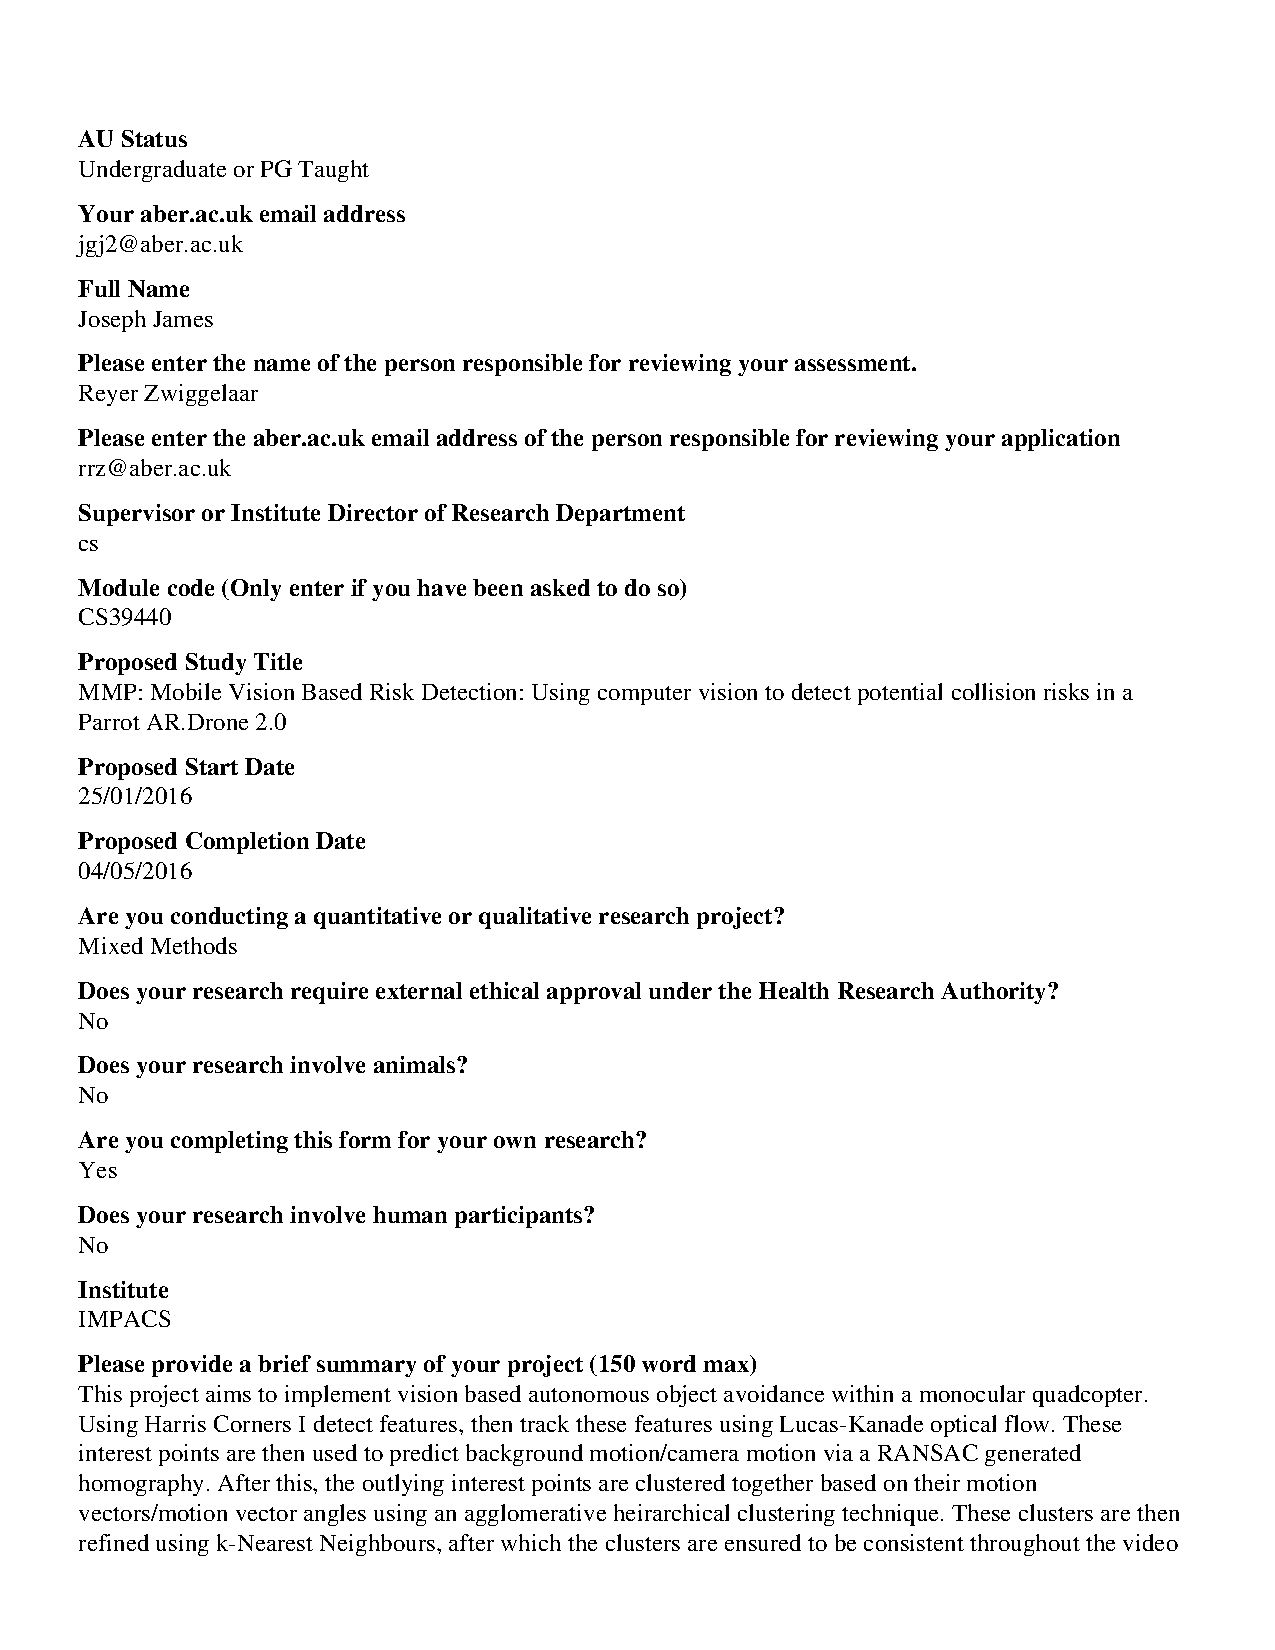
\includegraphics[scale=0.65]{Appendix2/4434.pdf}
\end{figure}
\clearpage
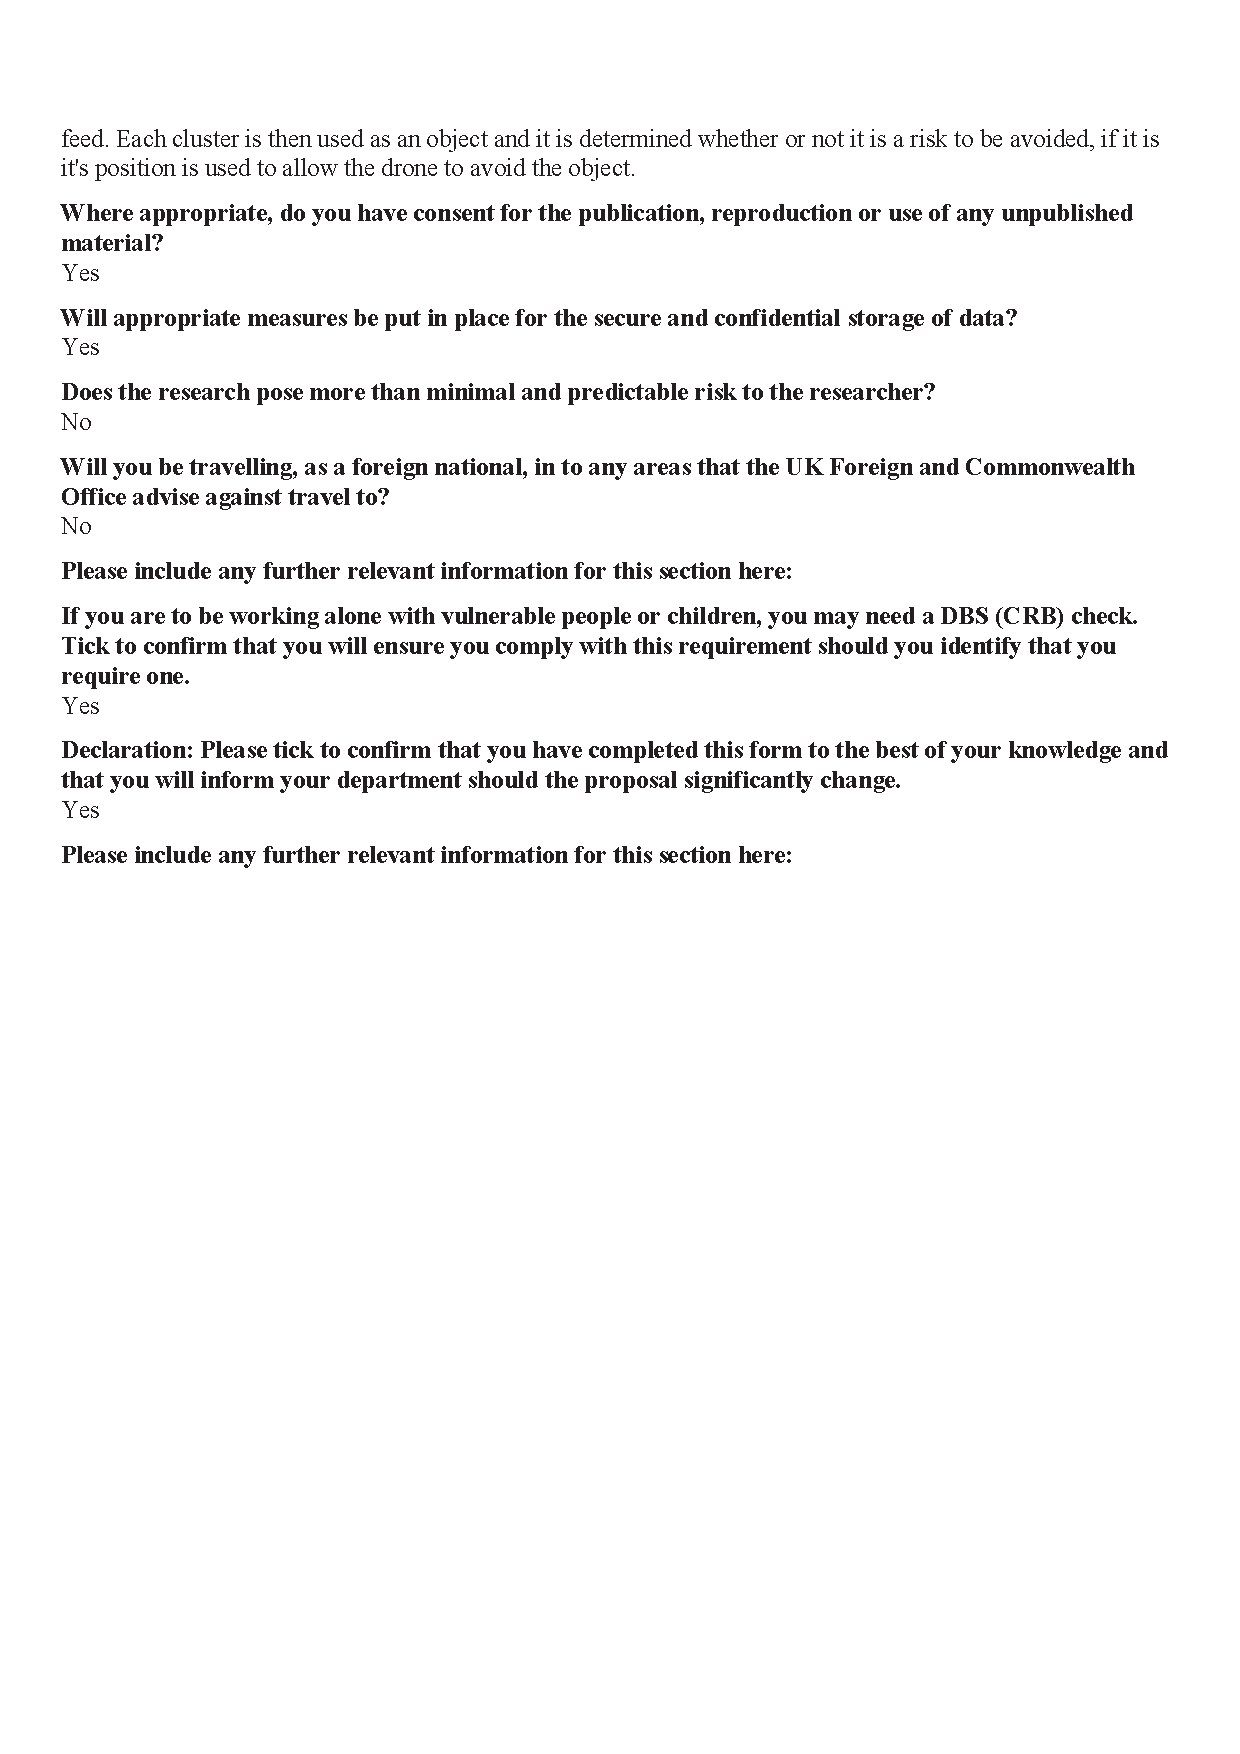
\includegraphics[scale=0.65]{Appendix2/4434(2).pdf}
\chapter{Code Examples}

\section{Interest Point struct}

The interest point data structure. Made to hold any and all information needed for each interest point.

\begin{verbatim}
 struct interestPoint {
   cv::Point2f currentFeature;
   cv::Point2f previousFeature;
   double MotionVectorAngle;
   bool isForeground;
   int clusterLabel;
 };
\end{verbatim}

\section{Clustering}
This is the clustering function I used for clustering my points.

\begin{verbatim}
/****************************************************************
 ****************************************************************
 ** Function: clusterPoints()                                   *
 ** Purpose : This function will perform the basics to start    *
 **             clustering the points.
 ** Params  : 							                        *
 ** Returns : 							                     	*
 ****************************************************************
*/
std::vector<cluster> clusterPoints(std::vector<interestPoint> *interestPoints, int splitLevel) {

  ///Sort the features in descending order based on number of occurences of corresponding motion vector angle
  mergeSort(*interestPoints);

  std::vector<cluster> allClusters;
  cluster current_cluster;
  current_cluster.centroid = interestPoints->at(0);
  current_cluster.label = 0;

  for (size_t i = 0; i < interestPoints->size(); i++) {
    if (std::abs(interestPoints->at(i).MotionVectorAngle - current_cluster.centroid.MotionVectorAngle) < angleThreshold) {
      current_cluster.interestPoints.push_back(interestPoints->at(i));
    }
    else {
      allClusters.push_back(current_cluster);
      current_cluster.centroid = interestPoints->at(i);
      current_cluster.interestPoints.clear();
      current_cluster.interestPoints.push_back(interestPoints->at(i));
      current_cluster.label = current_cluster.label + 1;
    }
  }

  return allClusters;

}
\end{verbatim}

\fancypagestyle{plain}{%
   \fancyhead{} %[C]{Annotated Bibliography}
   \fancyfoot[C]{{\thepage} of \pageref{LastPage}} % except the center
   \renewcommand{\headrulewidth}{0pt}
   \renewcommand{\footrulewidth}{0pt}
}

\setemptyheader

\nocite{*} % include everything from the bibliography, irrespective of whether it has been referenced.
	
% the following line is included so that the bibliography is also shown in the table of contents. There is the possibility that this is added to the previous page for the bibliography. To address this, a newline is added so that it appears on the first page for the bibliography. 
\addcontentsline{toc}{chapter}{Annotated Bibliography} % Adds References to contents page

%
% example of including an annotated bibliography. The current style is an author date one. If you want to change, comment out the line and uncomment the subsequent line. You should also modify the packages included at the top (see the notes earlier in the file) and then trash your aux files and re-run. 
%\bibliographystyle{authordate2annot}
\bibliographystyle{IEEEannot}
\renewcommand{\bibname}{Annotated Bibliography} 
\bibliography{References/joejames} % References file


\end{document}
